\chapter{Implementazione in {P}ython}
\section{Fase di estrazione e caricamento}
Per poter condurre una prima analisi esplorativa sul dataset preso in esame, il file originale \text{\emph{(public\_v2.json)}} è stato trasformato in un formato più adatto alla manipolazione e interrogazione rapida. In particolare, i passaggi principali sono stati:
\begin{itemize}
      \item Conversione in \emph{NDJSON}: Il dataset originale consiste in un unico oggetto JSON di grandi dimensioni, con chiavi univoche per ciascun log. Tramite il pacchetto Python \emph{ijson} è stata eseguita quindi una operazione di parsing in streaming, generando quindi un file di tipo \emph{NDJSON}, per il quale ogni riga rappresenta un singolo log strutturato. Per le finalità del caso studio si è deciso di mantenere il campo \emph{log\_id} per avere un riferimento univoco.
      \item Interrogazione tramite modulo DuckDB: Il file convertito viene quindi caricato in DuckDB, un database in-process molto efficiente per dataset di grandi dimensioni. Qui è stata effettuata una prima query di test per visualizzare un sottoinsieme di dati (limitato a 1000 righe) per velocizzare la fase esplorativa.
\end{itemize}

Osservando l'output prodotto dalla funzione df.info() di Pandas (libreria fondamentale nella data analysis e data exploration), emerge subito un primo dettaglio degno di nota. Sui primi 1000 risultati abbiamo 2 log che non hanno un method o una resource.
\begin{figure}[H]
      \centering
      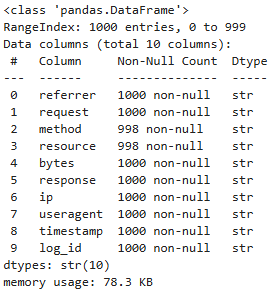
\includegraphics[width=0.5\textwidth]{Immagini/df_info_pandas.png}
      \caption{Output della funzione pd.DataFrame.info}
      \label{fig:df_info}
\end{figure}

Da una indagine più approfondita si constata che il server ha restituito response di tipo 400 (\emph{Bad Request}) e 408 (\emph{Request Timeout}), imputabili a cause di natura sia client-side, come richieste malformate o incomplete, sia server-side, come timeout dovuti a congestione o ritardi nella gestione della connessione, comportando quindi la mancata registrazione di alcuni campi essenziali come method e resource. Questa premessa ci permetterà una analisi più approfondita in seguito.

\section{Aggiunta al dataset di attacchi artificiali}

Al fine di testare la capacità di rilevamento del sistema, il dataset è stato integrato con dei record sintetici appositamente progettati per rappresentare minacce web esplicite. Tali istanze, pur mantenendo la coerenza strutturale con il traffico legittimo presente nel dataset, presentano anomalie semantiche riconducibili a pattern di attacco noti.

Di seguito si riporta un esempio di record configurato per simulare un attacco di tipo Cross-Site Scripting (XSS):



\begin{lstlisting}[language=json, caption={Esempio di log JSON con attacco XSS}, label={lst:xss_log}]
{
  "referrer": "http://search.lib.auth.gr/Search/<script>alert('XSS')</script>",
  "request": "search.lib.auth.gr:80 185.22.12.44 - - [01/Mar/2018:00:00:15 +0200] GET /Search?q=<script>alert('XSS')</script> HTTP/1.1 400 1200",
  "method": "GET",
  "resource": "/Search?q=<script>alert('XSS')</script>",
  "bytes": "1200",
  "response": "400",
  "ip": "185.22.12.44",
  "useragent": "Mozilla/5.0",
  "timestamp": "2018-02-28T22:00:15.000Z",
  "log_id": "attack_xss"
}
\end{lstlisting}

Per facilità di lettura, questi record sono stati catalogati con la voce \emph{attack} nel campo \emph{log\_id} in maniera tale da rendere più facile, in un successivo momento, l’estrazione degli stessi.

\section{Ingegneria delle feature}

Al fine di rendere il dataset interpretabile dall’algoritmo di Isolation Forest, quest’ultimo è stato sottoposto ad un processo di estrazione di nuove caratteristiche (\emph{features}). L’obiettivo è trasformare i log testuali in indicatori numerici e booleani che quantifichino anomalie strutturali, sintattiche e comportamentali nel traffico di rete.

Le feature prese in considerazione e riportate di seguito possono essere raggruppate sostanzialmente in tre macrocategorie: Analisi dimensionale, pattern matching e firme di attacco, analisi statistica e comportamentale


\begin{enumerate}
      \item Analisi dimensionale. \\
            Le anomalie nelle dimensioni indicano spesso tentativi di \emph{buffer overflow} o iniezioni di \emph{payload} estesi.

            \renewcommand{\labelenumii}{\theenumi.\arabic{enumii}}
            \begin{enumerate}
                  \item \texttt{resource\_len} (Lunghezza della risorsa):

                        Descrizione: Calcola il numero di caratteri che compongono la stringa della risorsa richiesta (\emph{URI}).

                        Razionale: Le richieste benigne tendono a raggrupparsi attorno a lunghezze standard \parencite{kruegel2003anomaly}. Poiché l'algoritmo Isolation Forest è progettato per identificare le anomalie isolando i campioni rari e dimensionalmente distanti (\emph{outlier}), fornire in input la lunghezza esatta della risorsa permette agli alberi di separare i \emph{payload} d'attacco con pochissimi split logici, aumentando l'efficienza computazionale e l'accuratezza del rilevamento.
                  \item \texttt{has\_suspicious\_request\_len} (Anomalia dimensionale della risorsa):

                        Descrizione: Applica il metodo statistico del Range Interquartilico (IQR) sulla lunghezza della risorsa. Assegna il valore 0 (normale) se la lunghezza rientra nell’intervallo
                        \begin{equation}
                              Q_1 - 1.5 \times \text{IQR} \le x \le Q_3 + 1.5 \times \text{IQR}
                        \end{equation}
                        e 1 (sospetto) in caso contrario.

                        Razionale: Fornisce al modello una classificazione pre-calcolata degli outlier unidimensionali, facilitando il partizionamento dei record palesemente anomali \parencite{kruegel2003anomaly}.
            \end{enumerate}
            % Fine sottolistap

      \item Pattern matching e firme di attacco (Analisi lessicale).\\
            Queste feature binarie (0/1) ricercano la presenza di sintassi associata a vettori di attacco noti o a strumenti di scansione automatizzata.

            \begin{enumerate}
                  \item \texttt{special\_char} (Conteggio dei caratteri speciali):

                        Descrizione: Conta le occorrenze di caratteri non alfanumerici (es. \texttt{<} \texttt{>} \texttt{'} \texttt{"} \texttt{\%} \texttt{;} \texttt{(} \texttt{)} \texttt{\{} \texttt{\}} \texttt{*} \texttt{+} \texttt{@}).

                        Razionale: Un'alta concentrazione di questi caratteri devia fortemente dalla baseline del traffico normale \parencite{kruegel2003anomaly}, fornendo all'Isolation Forest una metrica numerica netta per separare i payload malevoli.

                  \item \texttt{has\_traversal} (Rilevamento Path Traversal):

                        Descrizione: : Identifica la sequenza  \emph{../} nel corpo della richiesta.

                        Razionale: L’utilizzo della sequenza citata identifica un tentativo di risalita delle directory del server \parencite{owasp2021a01} \parencite{mitre_cwe22}.
                  \item \texttt{has\_sql\_keywords} (Rilevamento \emph{SQL Injection - SQLi}):

                        Descrizione: : Verifica la presenza di parole chiave tipiche del linguaggio SQL (\emph{union, select, insert, drop}) o tautologie (\emph{or 1=1, --, admin}).

                        Razionale: attacchi informatici come SQL Injection usano delle parole chiave che tentano di manipolare le query di backend del database \parencite{owasp2021a03}.

                  \item \texttt{has\_script\_tag} (Rilevamento \emph{Cross-Site Scripting - XSS}):

                        Descrizione: : Ricerca il tag \texttt{<script>} all’interno della richiesta.

                        Razionale: la ricerca mira ad identificare l’iniezione di codice eseguibile lato client, tipica degli attacchi XSS \parencite{owasp2021a03}.

                  \item \texttt{scanner\_agent} (Rilevamento \emph{User-Agent} malevoli):

                        Descrizione: Cerca stringhe associate a noti tool di vulnerability scanning o exploitation automatizzata (es. sqlmap, nikto, nmap, dirbuster, o l'uso base di curl).

                        Razionale: Gli strumenti di scanning automatici lasciano tracce estremamente evidenti, a meno che l’attaccante non compia sforzi deliberati per nasconderle. Ogni software che effettua richieste HTTP deve dichiararsi tramite l’header user-agent \parencite{nikto_useragent} \parencite{sqlmap_useragent} \parencite{nmap_useragent}.

                        L'efficacia della feature \emph{scanner\_agent} è supportata dalla natura stessa dei tool di \emph{vulnerability scanning}, i quali, nelle configurazioni predefinite, includono identificativi univoci all'interno dell'header \emph{HTTP User-Agent}. Tale comportamento è ampiamente documentato sia nelle specifiche tecniche degli strumenti stessi, sia nei set di regole dei principali Web Application Firewall che utilizzano queste “firme” per la chiusura immediata delle connessioni sospette.

                  \item \texttt{is\_known\_bot} (Identificazione di crawler e motori di ricerca tramite keyword):

                        Descrizione: Questa feature esegue una scansione del campo \emph{useragent} alla ricerca di stringhe identificative (\emph{keyword}) riconducibili a crawler benevoli e bot di indicizzazione (es. \emph{Googlebot, Bingbot, DotBot}).

                        Razionale: Durante le fasi preliminari di sperimentazione, è emerso che l'attività dei crawler generava un elevato numero di falsi positivi. Tali agenti automatizzati presentano profili di navigazione (frequenza di richiesta, esplorazione sistematica delle directory e parametri complessi) che l'Isolation Forest interpreta nativamente come anomalie. L'introduzione di questa feature permette al modello di pesare correttamente questo "rumore di fondo", distinguendo tra l'automazione finalizzata all'indicizzazione (benigna) e l'automazione finalizzata all'attacco (maligna).

            \end{enumerate}

      \item Analisi Statistica e Comportamentale.\\
            Queste metriche valutano il comportamento dell'utente e la risposta del server, fornendo un contesto più ampio rispetto alla singola riga di log.

            \renewcommand{\labelenumii}{\theenumi.\arabic{enumii}}
            \begin{enumerate}
                  \item \texttt{is\_error} (Codici di stato HTTP di errore):

                        Descrizione: Flag binario che indica se il server ha risposto con un codice di errore (status code $\geq$ 400)

                        Razionale: Gli attaccanti che effettuano brute-force o fuzzing, generano un'alta percentuale di risposte HTTP 400 (\emph{Bad Request}), 403 (\emph{Forbidden}) o 404 (\emph{Not Found}) \parencite{kruegel2003anomaly}.

                  \item \texttt{num\_params} (Complessità della Query String):

                        Descrizione: Conta il numero di parametri passati nella risorsa (contando il carattere =).

                        Razionale: Le pagine prese di mira per le iniezioni (SQLi, XSS) presentano spesso query string complesse per il passaggio dei payload \parencite{kruegel2003anomaly}. Più parametri sono presenti, maggiore è la probabilità che si tratti di una injection o tentativo di manipolazione.

                  \item \texttt{request\_per\_ip} (Frequenza di richiesta per host):

                        Descrizione: Calcola il numero totale di richieste effettuate da un singolo indirizzo IP rappresentando la densità di traffico generata da un singolo client.

                        Razionale: Valori anomali in questa metrica sono il sintomo primario di attacchi volumetrici \parencite{mitrebruteforce} \parencite{mitredos} \parencite{thottan2003anomaly}. Mentre le feature precedenti analizzano il contenuto, questa analizza quante richieste vengono fatte da un singolo indirizzo IP, rendendolo di fatto un parametro chiave per l’algoritmo nel distinguere utenti umani da script automatici.

                  \item \texttt{request\_entropy} (Entropia di Shannon della richiesta):

                        Descrizione: Calcola l'entropia della stringa di richiesta utilizzando la formula:
                        \begin{equation}
                              H(X) = - \sum_{i=1}^{n} p(x_i) \log_{2} p(x_i)
                        \end{equation}
                        Razionale: L'entropia misura il grado di "disordine" o casualità della stringa. Payload offuscati (es. codifica Base64), shellcode o stringhe generate algoritmicamente (DGA) presentano un'entropia significativamente maggiore rispetto alle normali URL legittime dove sono presenti parole di senso compiuto e strutture ripetitive \parencite{lyda2007using}

                        Nota Metodologica: Si osserva che nel dataset utilizzato per il presente caso studio, i campi testuali sono stati preventivamente sottoposti a un processo di hashing per ragioni di anonimizzazione e privacy. Poiché le funzioni di hash sono progettate per massimizzare la diffusione e produrre stringhe ad alta entropia indipendentemente dall'input originale, il valore di \texttt{request\_entropy} risulta uniformemente elevato per l'intero dataset. Pertanto, sebbene tale feature sia stata inclusa per completezza metodologica e per dimostrarne il valore predittivo in scenari di monitoraggio in chiaro (dove l'offuscamento malevolo si distingue nettamente dal testo naturale), nel contesto specifico di questo esperimento il suo apporto alla capacità discriminante dell'Isolation Forest è mitigato dalla natura crittografica dei dati sorgente.

                  \item \texttt{bytes\_ratio} (Rapporto di trasmferimento dati):

                        Descrizione: Calcola il rapporto tra i byte trasferiti in una specifica transazione e la media storica dei byte trasferiti per quella medesima risorsa.

                        Razionale: Mentre nel traffico ordinario la dimensione della risposta per una specifica risorsa URI tende a essere costante (bassa varianza), deviazioni significative nel volume di byte trasferiti indicano potenziali anomalie post-compromissione. Come evidenziato dal framework MITRE ATTACK nella tecnica T1020 (\emph{Automated Exfiltration}) \parencite{mitreT1020a}, il monitoraggio del volume cumulativo di dati permette di rilevare l'estrazione di informazioni sensibili tramite SQL Injection o accessi non autorizzati, rendendo tale rapporto un input critico per l'algoritmo di isolamento.



            \end{enumerate}

\end{enumerate}

\section{Applicazione dell'algoritmo}

L’algoritmo di Isolation Forest opera attraverso partizioni casuali dello spazio delle feature \parencite{liu2008isolation}; per questo motivo, il dataset è stato ridotto alle sole componenti numeriche e booleane derivate.

Sebbene l'algoritmo sia intrinsecamente invariante alla scala, è stato scelto di integrare un MinMaxScaler all'interno della pipeline di addestramento.

Nota Metodologica: L'uso della normalizzazione in questo caso studio non è dettato dai vincoli del modello di isolamento, ma dalla necessità di stabilizzare il processo di \emph{Hyperparameter Tuning}. Scalando le feature in un range $[0, 1]$, si garantisce che durante la fase di \emph{Grid Search} il calcolo delle metriche di scoring avvenga su una distribuzione controllata, facilitando la convergenza verso i parametri ottimali.

Per evitare una scelta arbitraria dei parametri (come la contamination o il numero di alberi), è stata implementata una ricerca sistematica tramite \emph{GridSearchCV}. Questo approccio trasforma un modello tipicamente non supervisionato in un sistema "guidato" dai dati reali (nel caso studio, gli attacchi inseriti manualmente).

\begin{itemize}
      \item Scoring Strategy: È stata scelta la \emph{recall\_macro} come metrica di riferimento (\texttt{refit='rec'}). In un contesto come quello del presente caso studio, è prioritario massimizzare il richiamo (\emph{Recall}), ovvero la capacità del sistema di non farsi sfuggire i veri attacchi, anche a costo di accettare un numero leggermente superiore di falsi positivi.
      \item Risultati dell'Ottimizzazione e Parametri ottimali:\\
            La configurazione ottimale identificata ha prodotto un Recall di $\sim$0.79 con i valori di \texttt{contamination} e \texttt{n\_estimators} impostati rispettivamente a 0.01 e 1000.
\end{itemize}

Un passaggio tecnico fondamentale riguarda la mappatura delle classi per la compatibilità con la libreria Scikit-Learn. Poichè l'Isolation Forest restituisce -1 per le anomalie e 1 per il traffico normale, le etichette del Ground Truth sono state allineate in tal senso.

\begin{lstlisting}[style=MatlabStyle, caption={}, label={lst:prova}]
    df['is_attack_real'] = df['log_id'].str.contains('attack').astype(int)
    df.loc[df['is_attack_real'] == 1, 'is_attack_real'] = -1
    df.loc[df['is_attack_real'] == 0, 'is_attack_real'] = 1
\end{lstlisting}

Questo allineamento permette alle funzioni di scoring della Grid Search di interpretare correttamente le anomalie come la classe di interesse da rilevare.

\section{Interpretazione dei risultati}

L'algoritmo Isolation Forest non restituisce un verdetto binario deterministico, bensì un valore di "anomalia" continuo. Mentre i punteggi negativi più profondi identificano record con feature multiple "fuori scala" (ovvero campioni che richiedono pochissimi partizionamenti per essere isolati), i punteggi prossimi allo zero rappresentano una zona di incertezza statistica dove solitamente ricadono i falsi positivi.

Si riporta di seguito un primo snippet di codice e la relativa tabella per verificare come l'algoritmo abbia classificato gli attacchi inseriti artificialmente nel dataset per testare la sensibilità del modello:

\begin{lstlisting}[style=MatlabStyle, caption={Verifica classificazione attacchi artificiali}, label={lst:interpretazione}]
df[df['log_id'].str.contains('attack')][['log_id', 'anomaly_score', 'scores']]
\end{lstlisting}

\begin{table}[H]
      \centering
      \begin{tabular}{|c|c|c|c|}
            \hline
            Index & log\_id           & anomaly\_score & scores    \\
            \hline
            1000  & attack\_xss       & -1             & -0.065746 \\
            1001  & attack\_sql       & -1             & -0.110561 \\
            1002  & attack\_traversal & -1             & -0.125805 \\
            1003  & attack\_scanner   & -1             & -0.138416 \\
            \hline
      \end{tabular}
      \caption{Scores per gli attacchi artificiali}
\end{table}


Come si evince dai risultati, tutti gli attacchi iniettati sono stati correttamente identificati come anomalie (\texttt{anomaly\_score = -1}), con punteggi di isolamento significativamente bassi, confermando l'efficacia delle feature estratte nel caratterizzare pattern malevoli noti.

Per convalidare il caso studio, si è proceduto al calcolo della matrice di confusione e del relativo \emph{classification report}. Questi strumenti sono essenziali per misurare la capacità del modello di distinguere tra traffico lecito e tentativi di intrusione.

\begin{figure}[H]
      \centering
      \includegraphics[width=\textwidth]{Immagini/Matrice\_di\_confusione.png}
      \caption{Matrice di confusione}
      \label{fig:mdc}
\end{figure}


\begin{lstlisting}[style=MatlabStyle, caption={Generazione del Classification Report}, label={lst:prova}]
from sklearn.metrics import classification_report
print(classification_report(df['is_attack_real'], df['is_attack_predicted']))
\end{lstlisting}

\begin{table}[H]
      \centering
      \begin{tabular}{|c|c|c|c|c|}
            \hline
            \dots        & precision & recall & f1-scores & support \\
            \hline
            0            & 1.00      & 0.99   & 1.00      & 998     \\
            1            & 0.36      & 1.00   & 0.53      & 4       \\

            accuracy     & -         & -      & 0.99      & 1002    \\
            macro avg    & 0.68      & 1.00   & 0.76      & 1002    \\
            weighted avg & 1.00      & 0.99   & 0.99      & 1002    \\

            \hline
      \end{tabular}
      \caption{Classification report}
\end{table}

L'analisi del report evidenzia una \textbf{Recall} del 100\% sulla classe 1 (attacchi), indicando che il modello non ha generato falsi negativi. Tuttavia, la \textbf{Precision} si attesta allo 0.36; questo valore, pur sembrando basso in un contesto di classificazione standard, è tipico dei sistemi di \emph{Anomaly Detection}. Come sottolineato da Sommer e Paxson \parencite{sommer2010outside}, nei sistemi di \emph{intrusion detection} basati su anomalie l’elevata incidenza di falsi positivi rappresenta uno dei principali limiti all’adozione in ambito operativo, in quanto attività lecite ma atipiche possono facilmente essere classificate come sospette.


Oltre agli attacchi artificiali, il modello ha catalogato come anomalie altri record presenti nel traffico originale. Di seguito vengono riportati i campioni con il punteggio di isolamento più basso:

\begin{lstlisting}[style=MatlabStyle, caption={Estrazione delle top anomalie}, label={lst:top_anomalies}]
top_anomalies = df[df['anomaly_score']==-1][['request','scores']].sort_values(by='scores')
\end{lstlisting}

\begin{table}[H]
      \centering

      \vspace{1mm}
      \resizebox{\textwidth}{!}{%
            \begin{tabular}{|c|p{20cm}|}
                  \hline
                  \textbf{Index} & \textbf{Request Log Entry}                                                                                                                                  \\ \hline
                  1003           & {\ttfamily search.lib.auth.gr:80 203.0.113.45 - - [01/Mar/2018:00:00:30 +0200] GET /wp-admin/install.php HTTP/1.1 404 250 - sqlmap/1.7}                     \\ \hline
                  1002           & {\ttfamily search.lib.auth.gr:80 91.200.12.77 - - [01/Mar/2018:00:00:25 +0200] GET /../../../../etc/passwd HTTP/1.1 403 300 - curl/7.58.0}                  \\ \hline
                  1001           & {\ttfamily search.lib.auth.gr:80 45.77.88.12 - - [01/Mar/2018:00:00:20 +0200] GET /login?user=admin' OR 1=1-- HTTP/1.1 500 800 http://evil.com Mozilla/5.0} \\ \hline
                  1000           & {\ttfamily search.lib.auth.gr:80 185.22.12.44 - - [01/Mar/2018:00:00:15 +0200] GET /Search?q=<script>alert('XSS')</script> HTTP/1.1 400 1200 ...}           \\ \hline
                  918            & {\ttfamily search.lib.auth.gr:80 176.92.34367 - - [01/Mar/2018:00:07:56 +0200] GET /Cover/Show?author=Winstanley... HTTP/1.1 200 677}                       \\ \hline
                  826            & {\ttfamily search.lib.auth.gr:80 176.92.34367 - - [01/Mar/2018:00:07:34 +0200] GET /Cover/Show?author=... HTTP/1.1 200 678}                                 \\ \hline
                  629            & {\ttfamily search.lib.auth.gr:80 155.207.36594 - - [01/Mar/2018:00:05:46 +0200] GET /Cover/Show?author=... HTTP/1.1 200 677}                                \\ \hline
                  497            & {\ttfamily search.lib.auth.gr:80 176.92.58901 - - [01/Mar/2018:00:05:08 +0200] GET / HTTP/1.1 200 4709 - Mozilla/5.0}                                       \\ \hline
                  429            & {\ttfamily search.lib.auth.gr:80 66.249.58337 - - [01/Mar/2018:00:04:25 +0200] GET /themes/jquerymobile/... HTTP/1.1 200 32415}                             \\ \hline
                  327            & {\ttfamily search.lib.auth.gr:80 85.74.35922 - - [01/Mar/2018:00:03:05 +0200] GET /themes/bootstrap3/... HTTP/1.1 200 65714}                                \\ \hline
                  59             & {\ttfamily search.lib.auth.gr:80 141.237.44390 - - [01/Mar/2018:00:00:19 +0200] GET /themes/bootstrap3/... HTTP/1.1 200 65714}                              \\ \hline
            \end{tabular}
      }
      \caption{Anomalie per punteggio di \emph{scores}}
\end{table}


Da un'analisi approfondita, emerge che tali richieste non appartengono al "rumore di fondo" generato dai crawler (correttamente filtrati dalla feature \\ \texttt{is\_known\_bot}), ma presentano valori di \texttt{resource\_len} e \texttt{bytes\_num} estremamente distanti dalla media. Ad esempio, le richieste ai temi grafici (Index 327, 59) o i file CSS/JS molto pesanti vengono isolati per la loro mole di dati. Nonostante la loro natura anomala dal punto di vista statistico, essi possono essere classificati come falsi positivi in ambito di sicurezza, rappresentando traffico lecito ma strutturalmente pesante.

\section{Applicazione dell'algoritmo all'intero dataset}

Nelle sezioni precedenti, al fine di condurre una fase esplorativa e calibrare i parametri dell’algoritmo, l’analisi è stata inizialmente limitata ai primi 1000 record del dataset.

Per verificare la tenuta del modello in uno scenario più realistico, l’algoritmo è stato successivamente applicato all’intero dataset. Questa seconda valutazione ha evidenziato uno dei principali limiti dell’Isolation Forest in contesti fortemente sbilanciati: i quattro attacchi inseriti manualmente non emergono più con sufficiente evidenza quando vengono immersi in un corpus di circa quattro milioni di record. In tale scenario, il modello attribuisce l’etichetta di anomalia a un numero molto elevato di osservazioni, circa 100.000, ma riflettono soprattutto traffico legittimo statisticamente atipico.

\begin{figure}[H]
      \centering
      \includegraphics[width=\textwidth]{Immagini/Matrice\_di\_confusione\_all.png}
      \caption{Matrice di confusione applicata all'intero dataset}
      \label{fig:mdcall}
\end{figure}

Dopo una più approfondita operazione di clustering ricavato dalla seguente query:

\begin{lstlisting}[style=MatlabStyle, caption={}, label={lst:topanomalies}]
    top_anomalies = df[df["anomaly_score"] == -1].sort_values(by='scores')
    top_anomalies_melted = top_anomalies.melt(
    id_vars='log_id',
    var_name='categories',
    value_vars=features_boolean,
    value_name='value')

active = top_anomalies_melted[top_anomalies_melted['value'] == 1]
combos = active.groupby('log_id')['categories'].agg(lambda x: ", ".join(tuple(sorted(x)))).reset_index(name='tuple')
\end{lstlisting}

Si estrapola la seguente tabella:

\begin{table}[H]
      \centering
      \begin{tabular}{|l|r|}
            \hline
            \textbf{Combinazione di Feature}                                         & \textbf{Frequenza} \\
            \hline
            is\_known\_bot, special\_chars                                           & 86.654             \\
            has\_suspicious\_request\_len                                            & 4.033              \\
            has\_suspicious\_request\_len, is\_known\_bot, special\_chars            & 3.011              \\
            has\_suspicious\_request\_len, is\_known\_bot                            & 2.879              \\
            is\_known\_bot                                                           & 2.556              \\
            has\_suspicious\_request\_len, is\_error                                 & 1.340              \\
            has\_sql\_keywords, has\_suspicious\_request\_len, is\_error             & 164                \\
            has\_suspicious\_request\_len, is\_error, is\_known\_bot                 & 131                \\
            is\_error, is\_known\_bot, special\_chars                                & 86                 \\
            has\_suspicious\_request\_len, special\_chars                            & 68                 \\
            is\_error, is\_known\_bot                                                & 34                 \\
            has\_sql\_keywords, has\_suspicious\_request\_len                        & 15                 \\
            is\_error                                                                & 4                  \\
            has\_suspicious\_request\_len, is\_error, is\_known\_bot, special\_chars & 1                  \\
            \hline
      \end{tabular}
      \caption{Report di classificazione delle occorrenze per combinazione di feature.}
\end{table}

L’analisi delle combinazioni di feature mostra che molte delle osservazioni segnalate come anomale condividono attributi ricorrenti come \emph{is\_known\_bot}, \emph{special\_chars} e \emph{has\_suspicious\_request\_len}. Questo suggerisce che il modello non sta isolando esclusivamente gli attacchi, ma intercetta anche pattern statistici frequenti nel traffico legittimo, in particolare richieste generate da crawler o risorse di dimensione insolita. Di conseguenza, l’anomalia rilevata dal modello non coincide sempre con un evento di sicurezza, ma spesso con una deviazione rispetto alla normalità statistica del dataset

Per visualizzare l’effetto del forte sbilanciamento del dataset, si riporta un grafico boxplot degli anomaly score rispetto alla posizione del record nel dataframe sia per il caso di un dataset limitato, sia per il caso del dataset completo.

\begin{figure}[H]
      \centering
      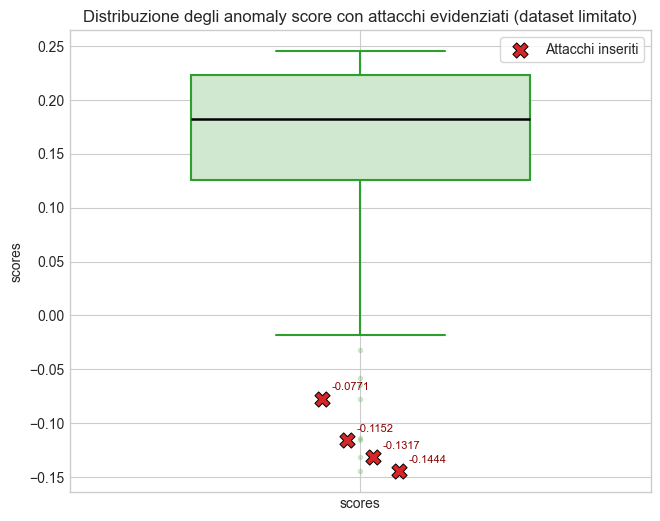
\includegraphics[width=\textwidth]{Immagini/boxplotlimited.png}
      \caption{Boxplot distribuzione anomalie (Dataset limitato ai primi 1000 record)}
      \label{fig:boxplotlimit}
\end{figure}

Per il dataset limitato, il boxplot mostra che i 4 attacchi cadono chiaramente nella zona di coda e vengono facilmente separati dalla distribuzione principale.

\begin{figure}[H]
      \centering
      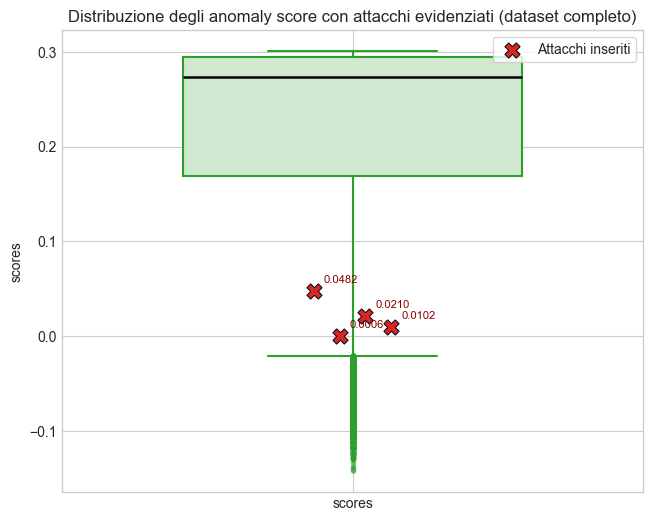
\includegraphics[width=\textwidth]{Immagini/boxplotall.png}
      \caption{Boxplot distribuzione anomalie (Dataset intero)}
      \label{fig:boxplotall}
\end{figure}

Per il dataset completo, la distribuzione degli score mostra uno sbilanciamento più accentuato e il segnale dei quattro attacchi perde forza discriminante, poichè la soglia di anomalia non li isola più in modo affidabile rispetto ai valori anomali dell'intero dataset.